% Preamble
\documentclass[12pt, a4paper]{article}
\usepackage[utf8]{inputenc}
\usepackage[english]{babel}

\usepackage{indentfirst}
\usepackage{rotating, graphicx}
\usepackage{geometry}
\usepackage{hyperref}
\usepackage{amsmath}
\usepackage{amssymb}
\usepackage{gensymb}
\usepackage{pdfpages}
\usepackage{color,soul}
\usepackage[justification=centering]{caption}
\newgeometry{vmargin={20mm}}

\usepackage[style=ieee]{biblatex}
\addbibresource{References.bib}

\usepackage{listings}
\usepackage{color}

\definecolor{dkgreen}{rgb}{0,0.6,0}
\definecolor{gray}{rgb}{0.5,0.5,0.5}
\definecolor{mauve}{rgb}{0.58,0,0.82}

\lstset{frame=tb,
	language=Java,
	aboveskip=3mm,
	belowskip=3mm,
	showstringspaces=false,
	columns=flexible,
	basicstyle={\small\ttfamily},
	numbers=none,
	numberstyle=\tiny\color{gray},
	keywordstyle=\color{blue},
	commentstyle=\color{dkgreen},
	stringstyle=\color{mauve},
	breaklines=true,
	breakatwhitespace=true,
	tabsize=3
}

\title{Final Year Project Progress Report}	
\author{Laurence Prins}
\date{25.05.2021}

\begin{document}
	\begin{center}
	\section*{\Huge Progress Report}
\end{center}

\vspace{60pt} \hfill \pagenumbering{gobble}

\noindent\textbf{Project Title:} E14 Indoor Positioning and Asset Tracking\\

\noindent\textbf{Academic Supervisor:} Shayne Crimp\\

\noindent\textbf{Student Name:} Laurence Prins\\

\noindent\textbf{Student ID Number:} 84063049\\

\noindent\textbf{Student Email:} ltp17@uclive.ac.nz\\

\pagebreak

\maketitle 

\pagebreak
\pagenumbering{arabic}
\section{Executive Summary}
To improve on the health and wellbeing of office space workers, a device is being developed which aims to provide employers with information on the office space. One such feature of the device is creating an indoor mapping system using sound. \\

The device will measure distance with up to 90\% accuracy and send the information back to a central node which can then generate a map at a user's request. Information from this map will be used to develop more ergonomic office environments for office space workers. \\

This project was split into four areas: the speaker subsystem, the microphone, sound propagation and sound detection. This report is concerned with the development of the speaker subsystem. \\

The speaker system consists of three major components: the speaker, the amplifier, and the microcontroller. The speaker itself is a high-fidelity audio device manufactured by PUI audio with part number AS01508MS-SP11-WP-R. This device has an 89dB sound pressure level (SPL) at 10cm with a 600Hz 2V peak waveform through it. \\

SPL is the measure of variation in atmospheric pressure due to sound, this can be related to two other sound measurements: sound power and sound intensity. Sound power is the rate at which sound is emitted from a source and sound intensity is the sound power per unit area. Sound intensity decreases with the square of the distance from the source, this is the inverse square law for sound. \\

Since the speaker requires more power input than the output of a microcontroller can output an amplifier is needed. Two amplifier circuits were built to compare, a class D amplifier using a PAM8403 and a class AB amplifier using an LM386. The class D amplifier can theoretically reach 92.75dB SPL. Testing needs to be done to confirm this and to compare the two amplifiers. Testing will also provide information on the pureness of the outputted waveform to see if further improvements need to be made to the system. \\

To control the speaker, a Teensy 4.0 microcontroller was programmed using the inbuilt Arduino tone function. This function produces a 50\% duty cycle PWM waveform at a given frequency. The board does not have an inbuilt digital to analogue converter, so for future development clever programming can be used to generate a sinusoidal PWM signal which is then filtered to form a sine wave. \\

\pagebreak
\tableofcontents
\pagebreak
\section{Project Overview}
Workers can spend up to 40 years of their lives within an office space environment. It is important for the worker's health and well-being if the office environment is as healthy as possible. The purpose of this project is to develop software to improve the ergonomics of office spaces using an indoor mapping system. The sponsor for this project is Wellnomics. \\

Wellnomics produces software solutions for improving the health and well-being of computer users. Software developed by Wellnomics include "Micro-pause and stretch break coaching" and "Human factors and ergonomics management reporting". A prototype device created by them is called a limpet shown in figure \ref{fig:limpetImage} which sits on a sit stand desk. The device takes measures of several environmental features such as the temperature of the office, the height of the sit stand desk etc. \\

\begin{figure}[!htb]
	\hfill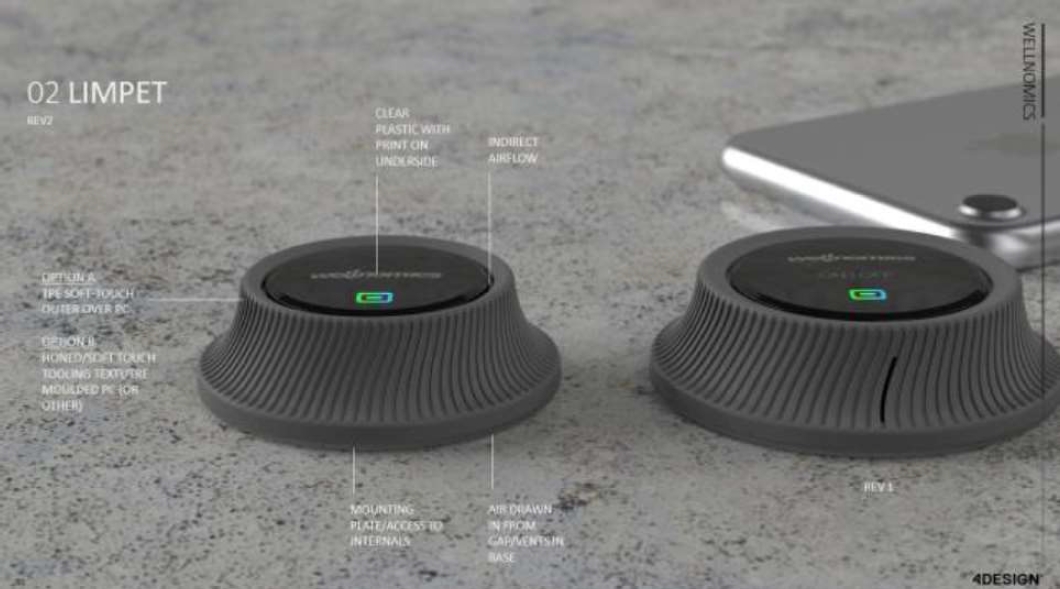
\includegraphics[width=\textwidth]{./Figures/Limpet_Image}\hspace*{\fill}
	\caption{'Limpet' device for sitting on desks within an office space, used to measure various office space features}
	\label{fig:limpetImage}
\end{figure}

The goal of this project is to use sound to do acoustic measurement between such devices. Since the speed of sound in air is known, by sending a pulse of sound and timing the time of travel between two points the distance can be calculated. If two devices are synced up, then by sending a pulse and timing the response an accurate measurement of distance can be produced. \\

The data from the acoustic measurements will be used to build a map of the office space with 100s of the devices attached to furniture. The measurements will be sent to a central node which will produce the map. Data from the map can be used to develop healthier office spaces. \\

This is not the first-time sound waves have been used for measuring distance. Use of SONAR for underwater navigation has been done, ultrasonics uses the time of arrival of sound to measure distance, even animals such as bats use echolocation. The challenge of this project is to develop a system which is capable of measuring distance within 90\% accuracy within an office environment and to produce a 3D map of the device locations. \\

To get accurate results a speaker system needs to be developed which can produce high fidelity sound with high output. This report will cover the development of the speaker system including research and development and the future development required for the rest of the project. \\

Alongside the speaker development there are three other areas being developed at the same time: the microphone, the sound propagation and edge detection. Once all these areas have been developed, the system can be tested for robustness in various environments. 
\pagebreak
\section{Progress to Date}
% =============================== Speaker Basics ====================================%
\subsection{Speaker Basics}
A speaker is an electromechanical transducer which converts electrical energy into mechanical energy in the form of acoustics \cite{whatLoudspeaker}. It consists of three major components: a permanent magnet, a voice coil, and a diaphragm. Figure \ref{fig:speakerExplodedView} shows an exploded view of a loudspeaker system, though the principles are the same for the surface mount speaker used in this project.\\
\begin{figure}[!htb]
	\hfill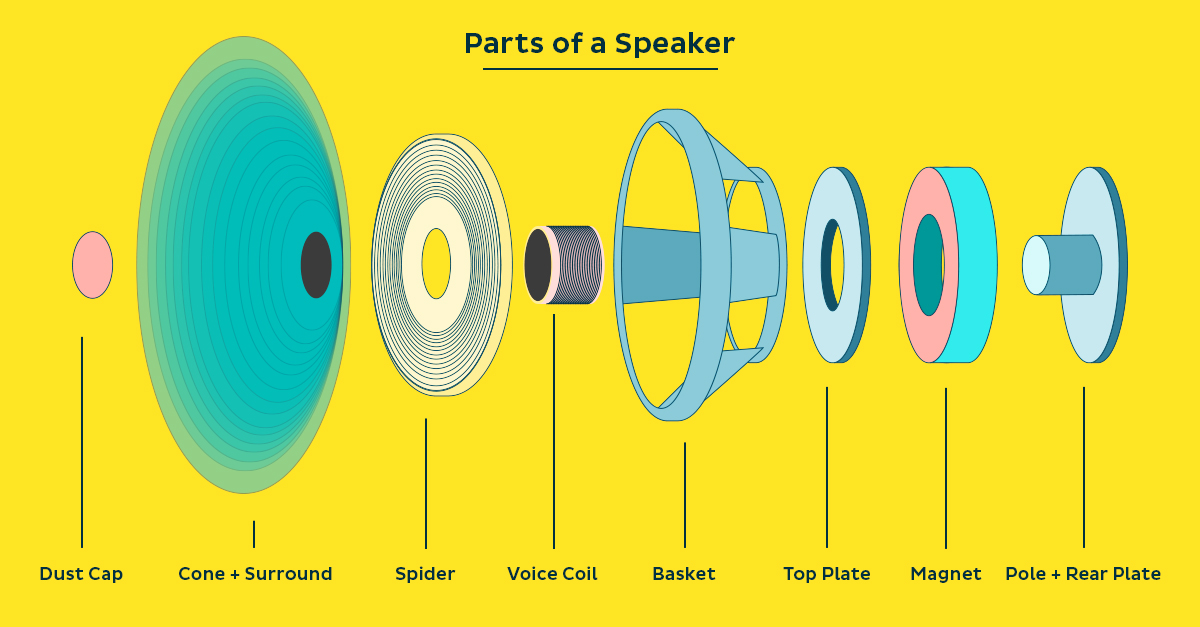
\includegraphics[width=\textwidth]{./Figures/parts_of_a_speaker}\hspace*{\fill}
	\caption{Parts of a speaker, source: \cite{howSpeaker}}
	\label{fig:speakerExplodedView}
\end{figure}\\
When current is passed through voice coil a magnetic force is induced on it by the permanent magnet. The force pushes or pulls the voice coil depending on the direction of the current \cite{whatLoudspeaker}. Any components attached to the voice coil will move with it, this includes the diaphragm. The role of the diaphragm is to perfectly mimic the movement of the voice coil to produce sound.\\

The block diagram for the speaker system is shown in figure \ref{fig:speakerBlockDiagram}. Research and development for each of these sections and the associated results is shown in the following sections.
\begin{figure}[!htb]
	\hfill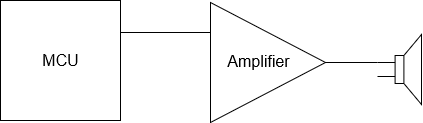
\includegraphics[width=0.5\textwidth]{./Figures/Speaker_Block_Diagram}\hspace*{\fill}
	\caption{Speaker system block diagram}
	\label{fig:speakerBlockDiagram}
\end{figure}
\subsection{Speaker}
% ============================= Speaker =========================================
The chosen speaker for this project is the AS01508MS-SP11-WP-R speaker. It has the specifications and frequency response shown in figure \ref{fig:speakerDataSheet}.\\ 
\begin{figure}[!htb]
	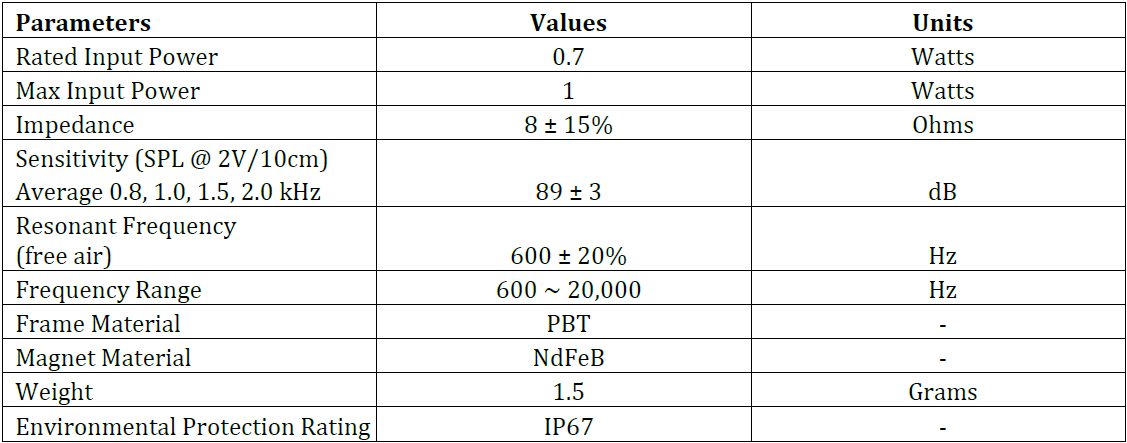
\includegraphics[width=0.55\textwidth]{./Figures/Speaker_Specifications}
	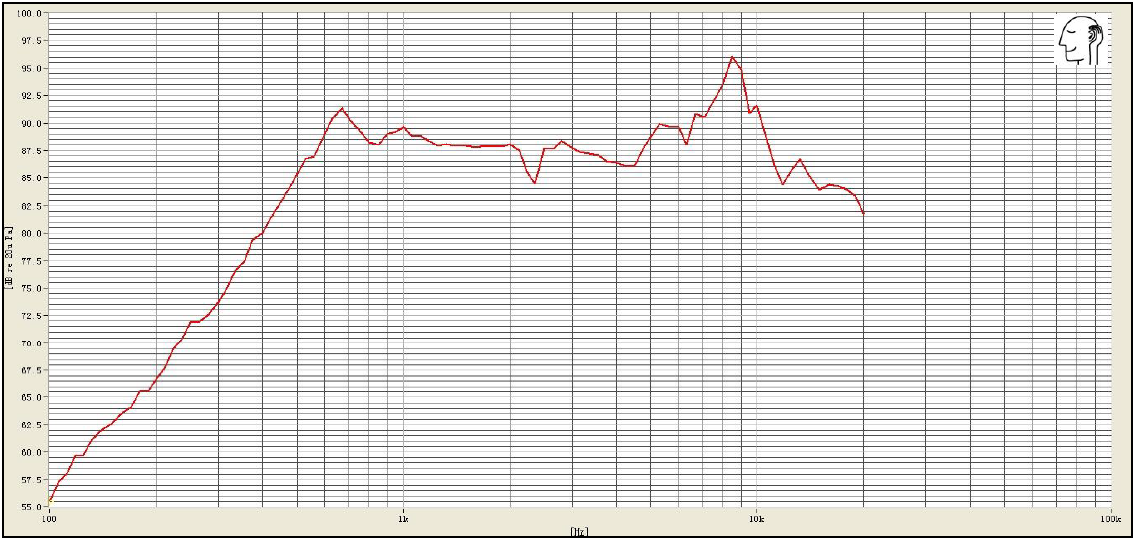
\includegraphics[width=0.45\textwidth]{./Figures/Speaker_Freq_Response}
	\caption{AS01508MS-SP11-WP-R specifications (left) and frequency response (right), source \cite{speakerDatasheet}}
	\label{fig:speakerDataSheet}
\end{figure}
% ================================ Sound Properties ==================================%
\subsection{Sound Parameters}
Understanding exactly what the information provided in the datasheet for the project requires an understanding sound parameters. The following section shows the major results of the research. 
\subsubsection{Sound Power}
Sound power is the rate at which sound energy is emitted from a source, generally given in decibels (dB). Sound power level (SWL) is given by \cite{soundTerminology}
\begin{equation}
	\label{eqn:SWL}
	L_W = 10log\left(\frac{P}{P_0}\right)
\end{equation}
\begin{center}
	\textit{P is the sound power of the source, $P_0$ is the reference sound power of $10^{-12}$ W which is the threshold of human hearing and $L_W$ is the SWL. }
\end{center}

\subsubsection{Sound Intensity}

Sound intensity is the measure of sound power per unit area. It is related to sound power by
\begin{equation}
	\label{eqn:soundIntensityGeneralForm}
	I(r) = \frac{P}{A(r)}
\end{equation}
\begin{center}
	\textit{Where A is the area of a sphere with area $4\pi r^2$ drawn at distance r.} 
\end{center}
Sound intensity decreases at a rate proportional to the inverse distance from the source. This is the inverse square law for sound mathematically represented by
\begin{equation*}
	I \propto \frac{1}{r^2}
\end{equation*}
This result can be used to determine the sound intensity between any two points from the same source \cite{audioParameters}
\begin{equation}
	\begin{aligned}
		\label{eqn:soundIntensityDistanceProperty}
		I_1r_1^2 = I_2r_2^2 \\
		\implies \frac{I_1}{r_2^2} = \frac{I_2}{r_1^2}
	\end{aligned}
\end{equation}
Sound intensity is also given in decibels given as the sound intensity level (SIL) \cite{soundTerminology}
\begin{equation}
	\label{eqn:SIL}
	L_I = 10log\left(\frac{I}{I_0}\right)
\end{equation}
\begin{center}
\textit{Where $L_I$ is the SIL and $I_0$ is the intensity threshold of human hearing, $10^{-12}$ $W/m^2$.}
\end{center}

\subsubsection{Sound Pressure}

Sound pressure is the average variation in atmospheric pressure caused by sound. Speakers give the sensitivity as sound pressure. Sound pressure level (SPL) is given in dB and can be calculated through \cite{soundTerminology}
\begin{equation}
	\label{eqn:SPL}
	L_P = 20log\left(\frac{P}{P_0}\right)
\end{equation}
\begin{center}
	\textit{Where $L_P$ is the Sound Pressure Level (SPL), P is the rms sound pressure in Pa and $P_0$ is the reference sound pressure equal to $2x10^{-5}Pa$ which is the threshold of human hearing.}
\end{center}
It is sound pressure which most devices such as microphones uses to detect sound. In typical depictions of sound waves, it is the sound pressure which is shown. In the datasheet for the speaker in figure \ref{fig:speakerDataSheet} the speaker sensitivity is given in sound pressure. Sound pressure and sound power can be related through the equation
\begin{equation}
	\label{eqn:soundPowerPressureRelation}
	L_W = L_P + 10log\left(\frac{A_s}{A_0}\right)
\end{equation}
\begin{center}
	\textit{where $A_s$ is an area of a surface which fully encompasses the source and $A_0$ = 1$m^2$}
\end{center}
With the speaker SPL known from the specifications in figure \ref{fig:speakerDataSheet}, the speaker audio power can be calculated using equation \ref{eqn:soundPowerPressureRelation}
\begin{equation}
	L_W = L_P + 10log\left(\frac{A}{A_0}\right) \therefore L_W = 89 + 10log\left(0.1 + (1/2)(0.0035)\right) = 77.2 \pm 3 dB
	\label{eqn:ourSpeakerPower}
\end{equation}
Which is a useful result for simulation. \\ 
% ============================= Amplifiers ======================================
\subsection{Speaker Amplifiers}
There are various classes of amplifiers which can take up the amplifier spot, the class is defined based on how much of the waveform the active component conducts. Two classes were considered for this project: class AB and class D. For more information on other classes and considerations see appendix A.\\
\subsubsection{Class AB Amplifier}
Class AB each active component operates for between half the wave and the full wave depending on the biasing of the diodes. An example of a class AB amplifier circuit diagram is given in figure \ref{fig:classABAmplifier}.\\

The chosen class AB amplifier for testing is the LM386. This was chosen as it is a low power, readily available amplifier. The current designed circuit for this amplifier is shown in figure \ref{fig:lm386Circuit} and the design choices are as followed\\
\begin{itemize}
	\item The 10k$\Omega$ variable resistor at the non inverting input acts as a volume knob, controlling the input voltage to the amplifier.
	\item The 10$\mu$F and 10k$\Omega$ connected between pins 1 and 8 control the amplifier gain, with the resistor set to 0$\Omega$ then the gain is set to 20, when the resistor is set to the full 10k$\Omega$ then the gain is set to 200.
	\item The 10$\mu$F ceramic capacitor connected to pin 7 is a bypass capacitor, it prevents high frequency noise from being amplified by the amplifier. 
	\item At the exit of pin 5 there is a 0.68$\mu$F film capacitor and a 10$\Omega$ forming a 'Zobel network'. High frequency signals (greater than 24.5kHz) are pulled to ground preventing damage to the speaker and also providing stability to the amplifier.
	\item The 220$\mu$F electrolytic capacitor before the speaker acts to remove the DC bias from the signal into the speaker. The capacitor forms a high pass filter with the 8$\Omega$ speaker, electrolytic capacitors are capable of having much higher capacitances than other capacitors, thus the capacitor here is chosen as electrolyic to allow the lower frequencies through. 
\end{itemize}

\begin{figure}[!htb]
	\hfill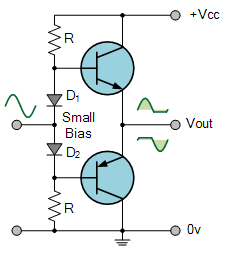
\includegraphics[width=0.3\textwidth]{./Figures/class_AB_amplifier}\hspace*{\fill}
	\caption{Class AB amplifier circuit diagram, source: \cite{amplifiers}}
	\label{fig:classABAmplifier}
\end{figure}
 
\begin{figure}[!htb]
	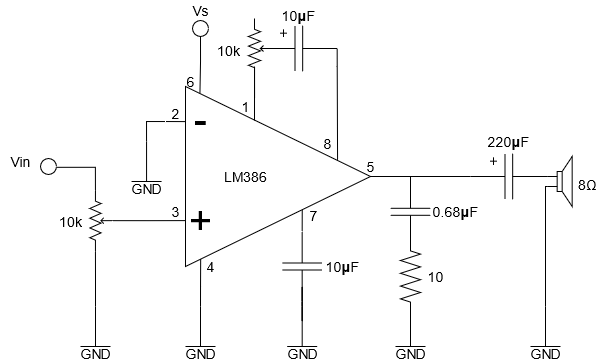
\includegraphics[width=0.5\textwidth]{./Figures/Class_AB_Amp}
	\includegraphics[width=0.5\textwidth]{./Figures/Class_AB_Amp_Physical}	
	\caption{Circuit diagram for the class AB amplifier circuit using the LM386 (left) and the physical implementation (right)}
	\label{fig:lm386Circuit}
\end{figure}

\subsubsection{Class D Amplifier}
Class D amplifiers are switching amplifiers. Where with the class AB amplifier the active components act as linear gain devices, class D amplifiers the active components act as switches. As a result, they are much more efficient since each transistor is either an on or off state and passes the full current, so there is very little power loss across the transistor. Theoretically a class D amplifier can reach 100\% efficiency. A block diagram for this class of amplifier and an example circuit is given in figure \ref{fig:classDAmplifierGeneral}. Here the inductors and capacitors form a low-pass filter which takes the sinusoidal PWM input and forms the amplified sine wave which is fed to the speaker. \\
\begin{figure}[!htb]
	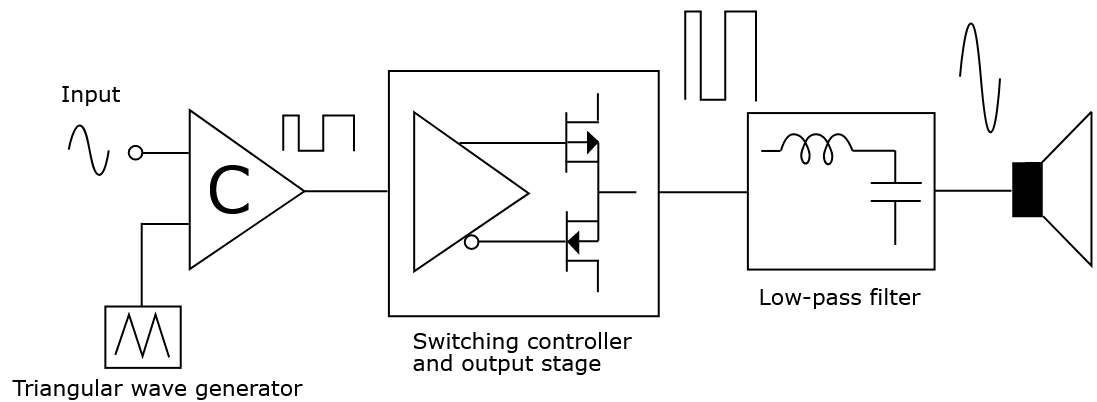
\includegraphics[width=0.55\textwidth]{./Figures/class_D_amplifier}
	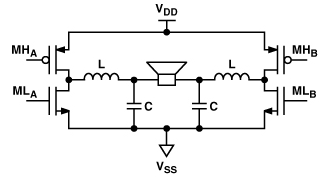
\includegraphics[width=0.45\textwidth]{./Figures/class_D_amplifier2}
	\caption{Class D amplifier block diagram (left) source: \cite{classDamplifier} and class D amplifier circuit diagram (right), \cite{classDamplifiercircuit}}
	\label{fig:classDAmplifierGeneral}
\end{figure}\\
The chosen class D amplifier for testing is the PAM8403 IC. This amplifier has efficiency of up to 90\%. This came on a pre-built circuit designed for use with Arduino with the part number XC4448 shown in figure \ref{fig:classDAmplifier}. The circuit takes a 5V power source and the input waveform and has outputs of up to 3W.
\begin{figure}[!htb]
	\hfill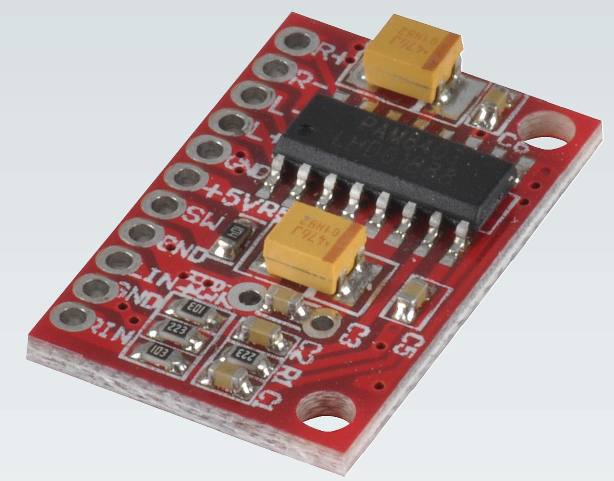
\includegraphics[width=0.4\textwidth]{./Figures/Class_D_Amp_Physical}\hspace*{\fill}
	\caption{Class D amplifier physical board}
	\label{fig:classDAmplifier}
\end{figure}\\
With the 5V power supply, the output waveform will be a 10V pk-pk waveform. The SPL for a 2V peak waveform across the speaker is average 89dB from figure \ref{fig:speakerDataSheet}. The 5V waveform is 2.5 times more input than this wave, based on the 3dB rule this will result in a SPL of 92.75dB at 10cm from the source. 

\subsection{Microcontroller and Code}
The chosen microcontroller is the Teensy 4.0. This has the benefit of a fast clock speed (up to 600Mhz) and is easily programmed using the Arduino IDE. Each pin has an output of 3.3V with 4mA maximum current. \\

The Arduino libraries come with an inbuilt 'tone' function which plays a 50\% duty cycle PWM waveform with a chosen frequency. Using this function, a piece of code was written which takes in a three-column array with the fields [freq, toneLength, number of pulses] and produces a tone with those properties. The code for this is shown in appendix B. This code can currently only play square wave tones.

\pagebreak
\section{Remaining Tasks}
The project has come to the end of the 14th week. Based on the Gantt chart produced in the project proposal shown in figure \ref{fig:ganttChart} the project is currently a week behind on the testing stage. The Gantt chart also shows the next steps in development. 
\begin{figure} [!htb]
	\hfill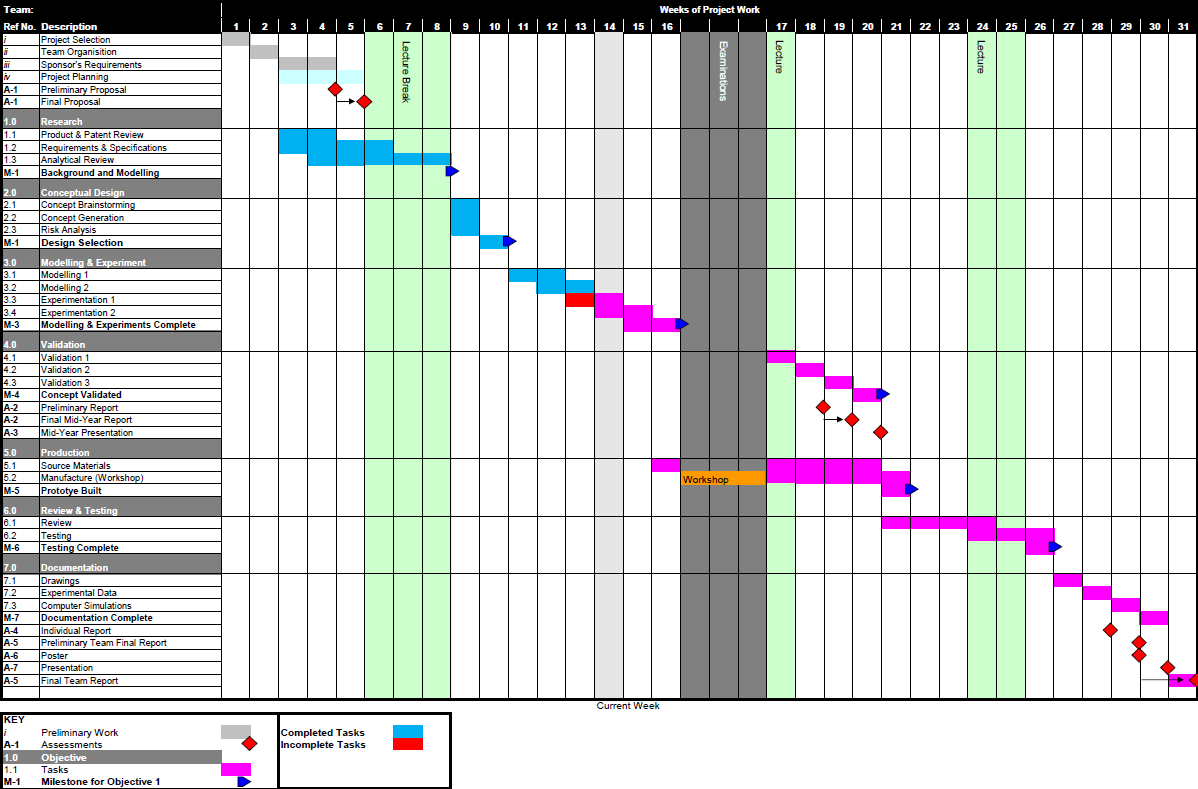
\includegraphics[width=\textwidth]{./Figures/Gantt_Chart}\hspace*{\fill}
	\caption{Gantt chart for project as made for the project proposal}
	\label{fig:ganttChart}
\end{figure}

The specific tasks for the speaker subsystem are as followed.
\subsection{More Waveforms}
The Teensy 4.0 microcontroller does not have an inbuilt DAC therefore the only waveform it can produce is a variation on a PWM waveform. A sinusoid wave could be produced by developing a method of producing sinusoidal PWM and implementing a low pass filter on the output of the amplifier. More waveforms could be produced following a similar method. The goal is to get this completed alongside testing and have it ready for the next stages of testing, so before June 6th.\\
\subsection{Testing}
\subsubsection{Sound Power and Pressure}
The speaker needs to be tested to verify whether the outputted sound pressure level matches the expected output. This needs to be done with both amplifiers to compare the differences between them. Testing can be done by connecting a microphone to an oscilloscope and analysing the waveform. If the output is vastly different compared to the theoretical then the circuit needs to be analysed to find points of improvement. Testing should be complete before June 14th.\\
\subsubsection{Waveform Purity}
The testing will reveal how pure the outputted waveform is. If the waveform has too much noise then a method of reducing this noise would need to be implemented into the speaker system. It is also necessary to know exactly what waveform is being produced as the receiver needs to know what to look for. This should be completed alongside testing so before June 14th. \\
\subsection{Budget Summary}
The current budget is summarised in table \ref{tab:budgetSummary}. This should be final budget until at least after the testing stage. After testing analysis will be done to see whether new components are necessary for improving the effectiveness of the devices and said components will be added to the budget summary. 
\begin{table} [!htb]
\begin{center}
	\caption{Budget Summary}
		\begin{tabular}{|c|c|c|c|}
			\hline
			Item & Cost & Amount & Total Cost (NZD) \\
			\hline
			Teensy 4.0 Board & 32.17 & 4 & 128.68 \\
			\hline
			MEMs microphone breakout & 12.25 & 5 & 61.25\\
			\hline
			Class D Amplifier (XC4448) & 5 & 2 & 10 \\
			\hline
			Total cost & & & 199.93\\
			\hline
		\end{tabular}
	
	\label{tab:budgetSummary}
\end{center}
\end{table}
\pagebreak
\section{Sustainability Analysis}
\subsection{Base Component Procurement}
\subsubsection{Silicon Semiconductors}
Silicon is mined as quartz ($SiO_2$), it is then refined into a metallurgical state and then refined again three more times into a 99.9999\% pure silicon wafer. Each step requires resources for production and results in wasted silicon. From the silica to the wafer require 2100kWh/kg to be manufactured into the pure state ready to be cut for the specific purpose \cite{siliconLCA}. The total amount of carbon emissions as a result is dependent on regional factors for how the power was produced.

\subsubsection{Battery}
Lithium button cell batteries are common batteries for use with portable electronics such as the system being developed for this project. The battery cell is constructed out of five components: the anode, cathode, separator, electrolyte and cell container \cite{BATTLCA_1}. The electrolyte material, lithium, is obtained from brine lake deposits and pegmatites.  Extraction of this is done through evaporating the salty water which leaves behind lithium carbonate ($Li_2CO_3$). This is done naturally so there is no carbon emissions and little impact on the environment. The lithium is then reacted with manganese oxide to produce material for use in batteries. The lithium production requires less energy than the production of the anode and cathodes \cite{BATTLCA_2}.
\subsubsection{Housing}
Assuming the housing is constructed using a 3D printer with polylactic acid or PLA. PLA is made from fermented plant starch such as corn, sugar cane etc. The growth of these plants requires land preparation, maintenance and harvesting which all have impacts on the environment be through power usage or chemicals. For sugarcane grown PLA, the total $CO_2$ emissions from growth to production is 501kg/ton PLA \cite{PLALCA_1}. PLA plastic produces less $CO_2$ emissions than other types of 3D printer materials when looking at the transportation costs \cite{PLALCA_2}.
\subsection{Usage}
Once the devices are installed in an office space the environmental impacts are considered based on the usage. The usage of the limpet devices can be broken down into operational requirements and maintenance. \\

Operational requirements involve the battery life of the lithium battery. The approximate lifespan of a lithium battery is 10 years \cite{usageLCA_1}. This is roughly the expected lifespan of the device which is advantageous. The use of a battery is advantageous form the usage point of view as the devices will not be drawing constant power from the mains supply, instead drawing from their own supply. \\

The devices will have impacts on the energy usage of the office spaces. Since employers are able to monitor the usage of desks within the building, they can set up the environment is such a way that the air conditioning or lighting is concentrated in areas of high use. This will reduce the energy usage across the entire office space which positively effects the environment. \\

If the device malfunctions then it is most likely to be replaced entirely since the repair of the device will cost more than a replacement. Repairing would require two way postage, whereas a replacement would only require single way postage producing less $CO_2$ from transportation. \\

\subsection{Distribution}
The developed devices could be sold individually or attached to desk shipped via freight ships. The environmental impact would then be dependent on the quantity of devices shipped together. Freight ships have a wide range of environmental impacts, including air pollution, spillage, ship-strikes on marine megafauna and ballast water containing aquatic invasive species \cite{WALKER2019505}. \\

Individually sold devices would need to be manually installed by the customer. Shipping these would be best done in bulk to the office. If shipped together then the effective impact per device can be kept down. Shipping many devices to a distributer would be the best option. From the distributer the devices could be placed onto a desk and reshipped. \\
\subsection{End of Life}
At the end of life most of the components can be recycled. The battery has all of its non-metal parts removed and the mixed metal is separated and the PCB is recycled using one of three methods: thermal recovering, chemical recovery, and physical recovery \cite{pcbRecycling_1}. \\

Thermal recovering involves heating the PCB to high temperatures which recovers the metals contained in the board. At high temperatures the fibreglass PCB material will burn off leaving behind the copper. The fibreglass material burns off into a toxic gasses.\\

Chemical recovery involves using acid to remove the fibreglass leaving behind the copper. This method results in large amounts of wastewater which needs treatment. With the increasing need for clean water all over the world, this is a poor option for recycling.\\

Physical recovery involves physically tearing the PCB materials apart leaving behind the copper. This has the least amount of environmental impact compared to thermal and chemical recovery. It has the negative that it is highly dangerous to those around.\\

The best choice of these recycling options is dependent on how well the recycling plant could manage the chemicals or the wastewater. Ultimately the best option for environmental sustainability is physical recovery if workers are equipped with sufficient PPE that prevents them from breathing in the harmful shards in the air. \\
\pagebreak
\section{Conclusions}
A speaker system was designed and built. The speaker chosen was the AS01508MS-SP11-WP-R speaker by PUI audio. It has a power output of 89dB SPL at 10cm using a 1kHz, 2V peak waveform. Using a class D amplifier this power output can theoretically reach 92.75dB if 5V is supplied to the amplifier. Testing is required to confirm this output and to verify the purity of the output waveforms.\\

A class AB amplifier was also constructed. Testing this and comparing it to the class D amplifier will help determine the best response. Once the speaker system has been tested individually, it will be ready to be tested in the full system. \\

The class D amplifier is theoretically much more efficient than the class AB amplifier. This is because the active components within the class D amplifer act as switches, passing the full current when in an on state. Class AB amplifiers the active components act as linear gain devices and are therefore active most of the time causing power loss. \\ 

The developed code takes a frequency, tone length, and number of pulses and produces a 50\% duty square wave with these properties. The Teensy 4.0 board used for the project does not have an inbuilt DAC so the only waves it can produce are square waves. A solution to this is to use clever programming to produce sinusoidal PWM output and pass this through a low pass filter. \\


\pagebreak
\printbibliography[title={References}]
\pagebreak
\section*{Appendix A}
\subsection*{Class A Amplifier}
In a class A amplifier, the output device conducts through the full waveform (360\degree). The most simple way to drive the speaker is to drive a BJT to control the input to the speaker this is shown in figure \ref{fig:speakerDriver1} (left). The circuit shown in figure \ref{fig:speakerDriver1} (right) shows a more complex class A amplifier which includes biasing and coupling and bypass capacitors to make a more reliable output. To operate for the full waveform, the transistor needs to be correctly biased such that it operates within its linear region.

\begin{figure} [!htb]
	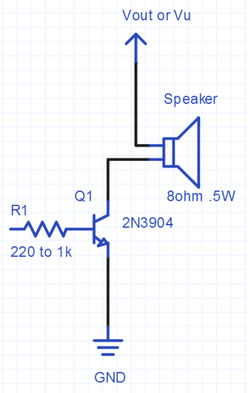
\includegraphics[width=50mm, scale=0.4]{./Figures/Speaker_Driver_1}
	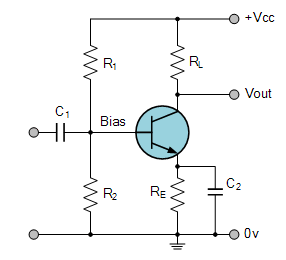
\includegraphics[scale = 1.0]{./Figures/class_A_amplifier_biasing}
	\caption{\textbf{Left:} simple speaker drive circuit. Source: \cite{speakerDriveSimple} \textbf{Right:} Class A amplifier circuit. Source: \cite{amplifiers}}.
	\label{fig:speakerDriver1}
\end{figure}
% ====================== Class B amplifiers	==============================
\subsection*{Class B Amplifier "Push Pull"}
Can improve on the efficiency of the class A amplifier by adding a complimentary pnp BJT. Class B amplifiers are defined based on each active component operating for half of the waveform (180\degree).  An example of a class B amplifier is given in figure \ref{fig:classBAmplifier} which also shows decoupling capacitors and resistors for correctly biasing the transistors. The npn transistor conducts for the positive half of the cycle and the pnp transistor conducts for the negative half of the waveform. At the zero-crossing point of the waveform, neither of the transistors will conduct and thus will end up having a deadzone causing distortion in the output waveform. \\
\begin{figure} [!htb]
	\hfill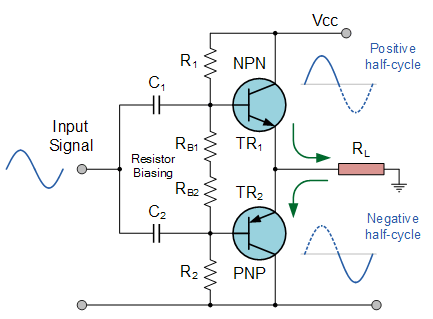
\includegraphics{./Figures/class_B_amplifier_biasing}\hspace*{\fill}	
	\caption{Class B amplifier circuit, source: \cite{amplifiers}}
	\label{fig:classBAmplifier}
\end{figure}\\
Neither of these two amplifiers discussed here are viable for audio amplification and thus this project. Class A is good for a quick method of interfacing with the microcontroller, however due to the power loss it is not good especially when there are better methods available. Class B has too much distortion at the zero crossing which is not good for a project where the waveform needs to be as precise as possible. This means the best of the options discussed is the class AB or the class D amplifiers.\\

\pagebreak
\section*{Appendix B}
The following is the current version of the code to produce a tone from the speaker, the serial read code was zombified from Robin2 code taken from the forum post on \url{https://forum.arduino.cc/t/serial-input-basics-updated/382007}.

\begin{lstlisting}
// Author: Laurence Prins
// Date: 13/05/2021
// Description: Initial testing of speaker driven from MCU

const byte numChars = 32;
char receivedChars[numChars];   // an array to store the received data
char tempChars[numChars]; 
char messageFromPC[numChars] = {0};

int toneFrequency = 1000; // Tone Frequency, default 1kHz
int toneLength = 1000; // tone duration, defaul 1 second
int pulses = 0; // Number of pulses, default 0

boolean newData = false;

int dataNumber = 0;             // new for this version

static int AUDIO_OUTPUT_1 = 3;

void setup() {
	// put your setup code here, to run once
	Serial.begin(9600);
}

void loop() {
	recvWithStartEndMarkers();
	if (newData == true) {
		strcpy(tempChars, receivedChars);
		// this temporary copy is necessary to protect the original data
		//   because strtok() used in parseData() replaces the commas with \0
		parseData();
		showParsedData();
		newData = false;
		generateBasicTone(toneFrequency, toneLength);
	}
}

void 
generatePulsedTone(int toneFrequency, int toneLength, int noPulses)
{
	for (int i = 0; i <= noPulses; i++) {
		generateBasicTone(toneFrequency, toneLength);
		delay(toneLength);
	}
}

void 
generateBasicTone(int toneFrequency, int toneLength) 
{
	tone(AUDIO_OUTPUT_1, toneFrequency);
	delay(toneLength);
	noTone(AUDIO_OUTPUT_1);
	
}

// Original code for reading from serial developed by Robin2
// source: https://forum.arduino.cc/t/serial-input-basics-updated/382007 
// Edited for use with the speaker code
void parseData() {      // split the data into its parts
	
	char * strtokIndx; // this is used by strtok() as an index
	
	strtokIndx = strtok(tempChars,","); // first index
	toneFrequency = atoi(strtokIndx); // convert to an integer
	
	strtokIndx = strtok(NULL, ","); // secondi index
	toneLength = atoi(strtokIndx); // convert to an integer
	
	strtokIndx = strtok(NULL, ","); // third index
	pulses = atoi(strtokIndx); // convert to an an integer
}

void recvWithStartEndMarkers() {
	static boolean recvInProgress = false;
	static byte ndx = 0;
	char startMarker = '[';
	char endMarker = ']';
	char rc;
	
	while (Serial.available() > 0 && newData == false) {
		rc = Serial.read();
		
		if (recvInProgress == true) {
			if (rc != endMarker) {
				receivedChars[ndx] = rc;
				ndx++;
				if (ndx >= numChars) {
					ndx = numChars - 1;
				}
			}
			else {
				receivedChars[ndx] = '\0'; // terminate the string
				recvInProgress = false;
				ndx = 0;
				newData = true;
			}
		}
		
		else if (rc == startMarker) {
			recvInProgress = true;
		}
	}
}

void showNewData() {
	if (newData == true) {
		Serial.print("This just in ... ");
		Serial.print(sizeof(receivedChars));
		newData = false;
	}
}

void showParsedData() {
	Serial.print("Frequency ");
	Serial.println(toneFrequency);
	Serial.print("Duration ");
	Serial.println(toneLength);
	Serial.print("Number of Pulses ");
	Serial.println(pulses);
}
\end{lstlisting}


\end{document}